%!TEX TS-program = xelatex
%!TEX encoding = UTF-8 Unicode

\documentclass[12pt]{article}
\usepackage{geometry}                % See geometry.pdf to learn the layout options. There are lots.
\geometry{a4paper,top=2cm}
\usepackage[parfill]{parskip}    % Activate to begin paragraphs with an empty line rather than an indent
\usepackage{graphicx}
\usepackage{amsmath}
\usepackage{amssymb}
\usepackage{mathtools}
\usepackage{physics}
\newcommand{\be}{\begin{equation}}
\newcommand{\ee}{\end{equation}}
\usepackage[thicklines]{cancel}
\usepackage{url}
\usepackage{booktabs}
\usepackage{csquotes}
\usepackage{qcircuit}
\usepackage{circledsteps}
\usepackage{nicefrac}
\usepackage{fontspec,xltxtra,xunicode}
\usepackage{xcolor}
\defaultfontfeatures{Mapping=tex-text}

\newcommand{\polv}{\ensuremath{\updownarrow}}
\newcommand{\polh}{\ensuremath{\leftrightarrow}}
\newcommand{\poldr}{\rotatebox[origin=c]{45}{\ensuremath{\leftrightarrow}}}
\newcommand{\poldl}{\rotatebox[origin=c]{-45}{\ensuremath{\leftrightarrow}}}
\newcommand{\bigzero}{\mbox{\normalfont\Large\bfseries 0}}

\title{Advanced Quantum Mechanics\\Class 24}
%\author{The Author}
\date{November 22, 2022}                                           % Activate to display a given date or no date

\begin{document}
\maketitle

\setcounter{section}{6}
%\setcounter{equation}{35}

\section{Approximation Methods}

%%% 01 OKAY

\setcounter{subsection}{2}
\subsection{Sudden and adiabatic approximations}

Often one faces a problem in which an
external field (or environment) changes
very quickly or very slowly over a
period of time $T$
$\Rightarrow$
the effects on the state of the system of
interest depend crucially on the
duration $T$ oves which the changes occur.

Let us suppose that the Hamiltonian $\hat{H}$ of the
system changes continuously in time from an
initial \emph{$\hat{H}_{0}$ at time $t_{0}$} to a \emph{$\hat{H}_{1}$ at time $t$}.

Put
\be
T=t_{1}-t_{0} \text { and } s=\frac{t-t_{0}}{T}
\ee
so
\be
t = t_0  +Ts
\ee
and parametrize the Hamiltonian $H(t)$ of the system
in terms of the ``dimensionless time'' $s$:
\be
\hat{H}(t) \rightarrow \hat{H}(s): \hat{H}(0)=\hat{H}_{0} \text{ and } \hat{H}(1)=\hat{H}_{1}
\ee

%%% 02 OKAY

To examine the evolution of the system from $t=t_{0}$
to $t=t_{1}$, it is convenient to use the time-evolution
operator $\hat{U}\left(t, t_{0}\right)$, writing it in terms of $s$:
\be
\hat{U}\left(t, t_{0}\right)=\hat{U}_{T}(s)
\ee
The evolution from $t_{0} \rightarrow t_{1}$ depends only on $T$;
$T$ measures the speed with which $\hat{H}$ changes from $\hat{H}_{0}$ to $\hat{H}_{1}$.
\emph{Speed of change:} $T$ large or small compared to some
system's intrinsic time scale%
\footnote{Always consider $T\sim T/\tau_0$, where $\tau_0$ is this intrinsic time scale (will be seen later).}%
.

Problem to be solved: to determine $\hat{U}\left(t_{1}, t_{0}\right)$,
that is, to determine $\hat{U}_{T}$ and examine its dependence on $T$
$\Rightarrow$ Results are simple in two limiting situations:

\begin{enumerate}
%
\item When $T \rightarrow 0$, rapid (sudden) passage: the dynamical
state of the system remains unchanged:
\be
\lim _{T \rightarrow 0} U_{T}(s)=1
\ee
%%% 03 OKAY
\item When $T \rightarrow \infty$, slow (adiabatic) passage: the system
passes from an eigenstate $|n, 0\rangle$ of $\hat{H}_{0}$ into an
eigenstate $|n, 1\rangle$ of $\hat{H}_{1}$ that derives from $|n, 0\rangle$
by the continuity of $\hat{H}(s)$.
\end{enumerate}



\subsubsection{Rapid passage -- sudden approximation}

We start from the Schrödinger equation for $\hat{U}\left(t, t_{0}\right)$ :
\be
i \hbar \frac{d \hat{U}\left(t, t_{0}\right)}{d t}=\hat{H}(t) \hat{U}(t, t_0), \quad \hat{U}(t_0, t_0)=1
\label{eq:g6}
\ee
This equation is equivalent to the integral equation:
\be
\int_{t_{0}}^{t} d t^{\prime} \frac{d \hat{U}\left(t^{\prime}, t_{0}\right)}{d t^{\prime}}=\frac{1}{i \hbar} \int_{t_{0}}^{t} d t^{\prime} \hat{H}\left(t^{\prime}\right) \hat{U}\left(t^{\prime}, t_{0}\right)
\ee
therefore
\be
\hat{U}\left(t, t_{0}\right)-\underbrace{\hat{U}\left(t_{0}, t_{0}\right)}_1%
=\frac{1}{i \hbar} \int_{t_{0}}^{t} d t \hat{H}\left(t^{\prime}\right) \hat{U}\left(t^{\prime}, t_{0}\right)
\ee
with
\[
t = t_0 + Ts
\begin{cases}
\begin{gathered}
dt = T ds\\
t^\prime = t \to s^\prime = s\\
t^\prime = t_0 \to s^\prime = 0
\end{gathered}
\end{cases}
\]
so finally
\be
\hat{U}_{T}(s)=1-\frac{i}{\hbar} T \int_{0}^{s} d s^{\prime} \hat{H}\left(s^{\prime}\right) U_{T}\left(s^{\prime}\right)
\label{eq:g9}
\ee

%%% 04 OKAY

For a sudden change in $\hat{H}$, the state of the system
remains unchanged: the second term in Eq.~\eqref{eq:g9}
goes to zero and
\be
\lim_{T \rightarrow 0} \hat{U}_{T}(s)=1
\label{eq:g10}
\ee
Now, for a nonzero $T$, Eq.~\eqref{eq:g10} can be considered
as the zeroth order approximation to a perturbative
expansion of $U_{T}(s)$ in which the expansion parameter
is $T$. That is, the system evolves from a state $\left|\psi_{0}\right\rangle$
at $s=0$ under the influence of a ``perturbation'' $\hat{H}(s)$
that is turned on at $s=0$, namely:
\be
\begin{gathered}
\hat{U}_{T}(s)=1-\frac{i}{\hbar} T \int_{0}^{s} d s^{\prime} \hat{H}\left(s^{\prime}\right)\\
+\left(\frac{i}{\hbar}\right)^{2} T^{2} \int_{0}^{s} d s^{\prime} \int_{0}^{s^{\prime}} d s^{\prime \prime} \hat{H}\left(s^{\prime}\right) \hat{H}\left(s^{\prime \prime}\right)+\ldots
\end{gathered}
\label{eq:g11}
\ee
If so, we need to quantify the error made in
truncating the series in Eq.~\eqref{eq:g11} to a finite
power in $T$. Here, let us examine the error
%%% 05 OKAY
made in truncating Eq.~\eqref{eq:g11} to $O\left(T^{2}\right)$, \textit{i.e.}
in using $U_{T}(s) \simeq 1$ for $T \neq 0$ $\Leftarrow$ \fbox{sudden approximation.}

The error can be estimated by calculating the
probability $\omega_{1}=\left\langle\overline{\psi}_{1} \mid \overline{\psi}_{1}\right\rangle$ of finding the system
at $s=1$ in a state $\left|\overline{\psi}_{1}\right\rangle$ \emph{other than $\left|\psi_{0}\right\rangle$},
\textit{i.e.} in the state
\be
\left|\overline{\psi}_{1}\right\rangle=\hat{Q}_{0}\left|\psi_{1}\right\rangle=\hat{Q}_{0} \hat{U}_{T}(1)\left|\psi_{0}\right\rangle
\ee
where
\be
\hat{Q}_{0}=1-\left|\psi_{0}\right\rangle\left\langle\psi_{0}\right|
\ee
projects out $\left|\psi_{0}\right\rangle$ from $U_{T}(1)\left|\psi_{0}\right\rangle=\left|\psi_{1}\right\rangle$,
and
we are supposing $\left\langle\psi_{0} \mid \psi_{0}\right\rangle=1$.

First, let us note that the lowest order term of $\omega_{1}$
is of $\mathcal{O}\left(T^{2}\right)$, given by
\[
\begin{aligned} 
\omega_{1}=\left\langle\overline{\psi}_{1} \mid \overline{\psi}_{1}\right\rangle 
&=\left\langle\psi_{1}\left|\hat{Q}_{0} \hat{Q}_{0}\right| \psi_{1}\right\rangle=\left\langle\psi_{1}\left|Q_{0}\right| \psi_{1}\right\rangle \\
&=\left\langle\psi_{0}\left|U_{T}^{\dagger}(1) \hat{Q}_{0} U_{T}(1)\right| \psi_{0}\right\rangle
\end{aligned}
\]
so
\[
U_{T}(1)=1-\frac{i}{h} T \int_{0}^{1} d s \hat{H}(s) \hat{U}_{T}(s)+(i / h)^{2} \int_{0}^{1} d s \int_{0}^{s} d s^{\prime} \hat{H}(s) \hat{H}\left(s^{\prime}\right)+\ldots
\]
and
%%% 06 OKAY
\be
\begin{aligned}
\omega_{1}
&=\left\langle\psi_{0}\left|\left(1+i / \hbar T \ldots\right) \hat{Q}_{0}(1-i / \hbar T \ldots)\right| \psi_{0}\right\rangle\\
&= \cancelto{0}{\bra{\psi_0}\underbrace{\hat{Q}_{0}\ket{\psi_0}}_{=0}}
-i/\hbar \cancelto{0}{T \int_0^1 \underbrace{\bra{\psi_0}\hat{Q}_{0}}_{=0}\hat{H}(s)\ket{\psi_0}}\\
&+i/\hbar \cancelto{0}{T \int_0^1 \bra{\psi_0}\hat{H}(s)\underbrace{\hat{Q}_{0}\ket{\psi_0}}_{=0}}\\
&+\frac{T^{2}}{\hbar^{2}} \int_{0}^{1} d s \int_{0}^{1} d s^{3}\bra{\psi_{0}}\hat{H}(s) \hat{Q}_{0} \hat{H}s^{\prime}\ket{\psi_{0}}
\label{eq:g14}
\end{aligned}
\ee
If we define
\be
\overline{H}=\int_{0}^{s} d s H(s)=\frac{1}{T} \int_{t_{0}}^{t} d t^{\prime} \hat{H}\left(t^{\prime}\right)
\label{eq:g15}
\ee
one can write Eq.~\eqref{eq:g14} as
\[
\begin{aligned} 
\omega_{1} 
&=\frac{T^{2}}{\hbar^{2}}\left\langle\psi_{0} \mid \overline{H} \hat{Q}_{0} \overline{H} \mid \psi_{0}\right\rangle
=\frac{T^{2}}{\hbar^{2}}\left\langle\psi_{0}\left|\overline{H}\left(1-| \psi_{0}\right\rangle\left\langle\psi_{0}\right|\right) \overline{H} \mid \psi_{0}\right\rangle \\ 
&=\frac{T^{2}}{\hbar^{2}}\left[\left\langle\psi_{0}\left|\overline{H}^{2}\right| \psi_{0}\right\rangle-\left(\left\langle\psi_{0}|\overline{H}| \psi_{0}\right\rangle\right)^{2}\right] 
\end{aligned}
\]
so
\be
\omega_1 = \frac{T^2}{\hbar^2} \left(\Delta\overline{H}\right)^2
\ee

%%% 07 OKAY

Validity of the sudden approximation requires
\be
\omega_1 \ll 1 \Rightarrow \boxed{T \ll \frac{\hbar}{\Delta\overline{H}}}\,, 
\Delta\overline{H} = \sqrt{(\Delta\overline{H})^2}
\ee
\begin{quote}
\emph{Meaning:} nothing happens to the initial state
in a time interval $\hbar/ \Delta \overline{H}$ while the
system is governed by the time-averaged
Hamiltonian $\overline{H} \leftarrow$ Eq.~\eqref{eq:g15}.
\end{quote}

\subsubsection{Adiabatic passage -- adiabatic approximation}

We initially establish the \emph{adiabatic theorem}
$\rightarrow$ we limit the discussion to the discrete
spectrum of the Hamiltonian $\hat{H}$.

Let $\ket{n,t}$ be the instantaneous eigenstates of
$\hat{H}(t)$, that is:
\be
\hat{H}(t)|n, t\rangle=E_{n}(t)|n, t\rangle
\ee
%
\be
\hat{P}_{n}(t)=|n, t\rangle\langle n, t|, n=1,2, \ldots
\ee

%%% 08 OKAY

We \emph{assume} that:
\begin{enumerate}
\item $\hat{H}(t),|n, t\rangle, E_{n}(t)$ are continuous functions of $t$
%
\item The eigenvalues $E_{n}(t)$ remain distinct
during the entire time interval $T=t-t_{0}$:
\[
E_{n}(s) \neq E_{m}(s), \forall\, n, m
\begin{cases}
\begin{gathered}
\text{\emph{gap} between consecutive}\\
\text{eigenvalues, non crossing}
\end{gathered}
\end{cases}
\]
%
\item The derivatives $\frac{d\hat{P}_n(t)}{dt}$ and$ \frac{d^2\hat{P}_n(t)}{dt^2}$ are well
defined and piece-wise continuous in $T=t-t_0$
\end{enumerate}
%
In terms of the variable $s$, the Schrödinger equation
for $\hat{U}\left(t, t_{0}\right)$ in Eq.~\eqref{eq:g6} is given by
\be
i \hbar \frac{d U_{T}(s)}{d s}=T \hat{H}(s) \hat{U}_{T}(s)
\label{eq:g20}
\ee
and the Hamiltonian can be written as
\be
\hat{H}(s)=\sum_{n} E_{n}(s)|n, s\rangle\langle n, s|=\sum_{n} E_{n}(s) \hat{P}_{n}(s)
\ee
The adiabatic theorem states that, under assumptions 1), 2), 3):
\be
\boxed{
\lim_{T \rightarrow \infty} \hat{U}_{T}(s) \hat{P}_{n}(0)=
\hat{P}_{n}(s) \lim_{T \rightarrow \infty} \hat{U}_{T}(s)
}
\ee

%%% 09 OKAY

Meaning of the theorem: suppose at $s=0$ $(t=t_0)$ the
state of the system is $\ket{n,0}$, an eigenstate of $\hat{H}_0$. At time
$s$ for $T \to \infty$, the state $\displaystyle\ket{\psi(s)}_\infty = \lim_{T\to\infty} \ket{\psi(s)}$ is given by:
\be
\begin{gathered}
\ket{\psi(s)}_\infty = \lim_{T\to\infty} \ket{\psi(s)} = 
\lim_{T\to\infty} \hat{U}_{T}(s) \ket{\psi(0)} = \lim_{T\to\infty} \hat{U}_{T}(s) \ket{n,0}\\
= \lim_{T\to\infty} \hat{U}_{T}(s) \hat{P}_{n}(0) \ket{n,0} = \underbrace{\hat{P}_{n}(s)}_{\op{n,s}} \lim_{T\to\infty} \hat{U}_{T}(s) \ket{n,0}\\
= \ket{n,s} \lim_{T\to\infty} \bra{n,s} \hat{U}_{T}(s) \ket{n,0} = \bra{n,s} \hat{U}_{T}(s) \ket{n,0}_\infty \ket{n,s}
\end{gathered}
\ee
That is, $\ket{\psi(s)}_\infty$ is an eigenstate of $\hat{H}(s)$ with eigenvalue
$E_n(s)$: under an \emph{infinitely slow evolution} (\textit{i.e.} $T\to\infty$)
the system remains in an instantaneous eigenstate
of $\hat{H}(s)$. Since the evolution is unitary, the norm is
preserved, $|{}_\infty\!\bra{\psi(s)}\ket{\psi(s)}_\infty\!|$ = $|\bra{n,0}\ket{n,0}|$ = 1. Therefore
\be
\lim_{T\to\infty} \bra{n,s}U_{T}(s)\ket{n,0} = e^{-i\varphi_n(s)}
\ee
and
\be
\lim_{T\to\infty} \op{\psi(s)} = \op{n,s} = \hat{P}_n(s)
\ee

\emph{Trivial example:} $\hat{P}_n(s) = \op{n,s} \overset{(!!!)}{=} \op{n,0} = \hat{P}_n(0)$.
In this case, the instantaneous Hamiltonian is given by:
%%% 10 OKAY
\[
\hat{H}(s) = \sum_n E_n(s) \op{n,s} = \sum_n E_n(s) \hat{P}_n(s) = \sum_n E_n(s) {P}_n(0)
\]
meaning that $[\hat{H}(s),\hat{H}(s^\prime)] = 0$ $\Leftarrow$ valid for any $T$, \emph{therefore
valid for $T\to\infty$}. Therefore, one can integrate Schrödinger's equation, Eq.~\eqref{eq:g20}, exactly:
\[
\begin{gathered}
\hat{U}_T(s) = \mathcal{T} e^{-i / \hbar T \int_{0}^{s} d s^{\prime} \hat{H}(s^{\prime})} = 
1 -i / \hbar T \int_{0}^{s} d s^{\prime} \hat{H}(s^{\prime})\\
+\frac{1}{2!}(i/\hbar T)^2 \int_{0}^{s} d s^{\prime} \int_{0}^{s} d s^{\prime\prime}
\underbrace{\mathcal{T} [\hat{H}(s^\prime) \hat{H}(s^{\prime\prime})]}_{\Circled{1}}
+\ldots
\end{gathered}
\]
but in \Circled{1}, since $[\hat{H}(s^\prime),\hat{H}(s^{\prime\prime})] = 0$, the
time-ordering operator $\mathcal{T}$ is not necessary 
(remember $\mathcal{T}[A(t_1)B(t_2)] = A(t_1)B(t_2)$ if $t_1 > t_2$, 
$B(t_2)A(t_1)$ otherwise).
So:
\be
\begin{aligned}
\hat{U}_T(s) 
&=1 -i / \hbar T \int_{0}^{s} d s^{\prime} \hat{H}(s^{\prime})
+\frac{1}{2!}(i/\hbar T)^2 \left(
	\int_{0}^{s} d s^{\prime} \hat{H}(s^{\prime})
\right)^2+\ldots\\
&= e^{-i / \hbar T \int_{0}^{s} d s^{\prime} \hat{H}(s^{\prime})}
 = e^{-i / \hbar T \int_{0}^{s} d s^{\prime} E_n (s^{\prime}) \hat{P}_n}\\
&= \sum_n e^{-i / \hbar T \int_{0}^{s} d s^{\prime} E_n (s^{\prime})} \hat{P}_n,\\
&\text{where we use that } \hat{P}_n(s) = \hat{P}_n(0) \equiv \hat{P}_n
\end{aligned}
\ee
so finally
\be
\boxed{
\hat{U}_T(s) = \sum_n e^{-i \varphi_n(s)} \hat{P}_n, \text{ with }
\varphi_n(s) = (1/\hbar){T} \int_0^s ds^\prime E_n(s^\prime)
}
\ee
%%% 11 OKAY
Therefore:
\[
\ket{\psi(s)} = \hat{U}_T(s) \ket{\psi(0)}, \ket{\psi(0)} = \ket{n,0}
\]
so
\be
\ket{\psi(s)} = \hat{U}_T(s) \ket{n,0} 
= \sum_{n^\prime} e^{-i\varphi_{n^\prime}(s)}\hat{P}_{n^\prime} \ket{n,0}
= e^{-i\varphi_{n}(s)} \ket{n,0}
\ee
But remember that $\ket{\psi,s}$ is an eigenstate of $\hat{H}(s)$:
\be
\begin{aligned}
\hat{H}(s)\ket{\psi,s} 
&= \sum_{n^\prime} e^{-i\varphi_{n^\prime}(s)}
\underbrace{\hat{H}(s)\hat{P}_{n^\prime}}_{E_{n^\prime}(s)\hat{P}_{n^\prime}} \ket{n,0}
 = \sum_{n^\prime} E_{n^\prime}(s) e^{-i\varphi_{n^\prime}(s)} \hat{P}_{n^\prime} \ket{n,0}\\
&= E_n(s) e^{-i\varphi_{n}(s)} \ket{n,0} = E_n(s) \underbrace{\ket{\psi(s)}}_{\ket{n,s}}
\end{aligned}
\ee
$\Rightarrow$ 
If, at $t=t_{0}$, $|\psi(t_{0})\rangle$ is an eigenstate of $\hat{H}(t_{0})$
$|n, t_{0}\rangle$ with eigenvalue $E_{n}(t_{0})$, at $t=t_{1}$ $|\psi(t)\rangle$
is an eigenstate from $H(t_{1}),|n, t_{1}\rangle$, which differs
from $|n, 0\rangle$ by a phase factor
%
\be
e^{-i / \hbar \int_{t_{0}}^{t_{1}} d t^{\prime} \hat{H}\left(t^{\prime}\right)}
\ee
%
\begin{quote}
$\Rightarrow$\emph{Recall:} this is valid under the 
\emph{(drastic)} assumption
$[\hat{H}(t), \hat{H}(t^{\prime})]=0$
\end{quote}

\setcounter{equation}{65}
Now, for \emph{$T$ finite}, setting
\be
\hat{U}_T(s) \hat{P}_n(0) = \hat{P}_n(s) \hat{U}_T(s)
\ee
is an approximation, the \emph{adiabatic approximation}.

\emph{Next:} examine the adiabatic aproximation
and consider cyclic motions $\Rightarrow$ Berry phase.
We will abandon the analysis in terms of
variables $s$ and $T$. We will also parameterize
the ``environment'' in terms of coordinates
of a manifold.

%%% PUXADO DA AULA 25

Suppose a quantum system in contact with a \emph{time-dependent}
environment, \textit{e.g.} an external field, or the system
is part of a larger system, etc. Let $R_{1}(t), R_{2}(t), \ldots$
be parameters that characterize the environment.
\begin{itemize}
\item the Hamiltonian $\hat{H}$ and observables $\hat{A}$ of the quantum
system depend on $\vec{R}(t)=\left(R_{1}(t), R_{2}(t), \ldots\right)$;
\item each value of $\vec{R}(t)$ characterizes a particular
configuration of the environment
\item changes in $\vec{R}(t)$ describe a curve
in some manifold $\Rightarrow$ ``parameter space'' $M$
\end{itemize}

\emph{Assumption:} $\hat{H}=\hat{H}(\vec{R})$ and $\hat{A}=\hat{A}(\vec{R})$ are \mbox{\emph{smooth} and \emph{single-valued} functions of $\vec{R}$}.

%%% 01 OKAY

\emph{Example:}
\begin{itemize}
\item System: quantum magnetic moment,
 described by an operator $\hat{\vec{\mu}}$
\item Environment: time-dependent magnetic field
$\vec{B}(t)$, with constant magnitude $B=|\vec{B}|$
\end{itemize}

\begin{minipage}{0.6\textwidth}
\setcounter{equation}{77}
Hamiltonian of the system is then
\be
\hat{H}(t)=-\hat{\vec{\mu}} \cdot \vec{B}(t)=-g \underbrace{\frac{q}{2 m c}}_{\text{note the c}} \hat{\vec{J}} \cdot \vec{B}
\ee	
Defining the ``coordinates'' $\vec{R}(t)=B \hat{R}(t)$ and
\be
b=-g \frac{q}{2 m c} B
\ee
one can write $\hat{H}$ as
\be
\hat{H}(t)=\hat{H}(\vec{R}(t)) \equiv \hat{H}(R)=b \hat{R}(t) \cdot \hat{\vec{J}}
\label{eq:g80}
\ee
\end{minipage}%
\begin{minipage}{0.4\textwidth}
\hfill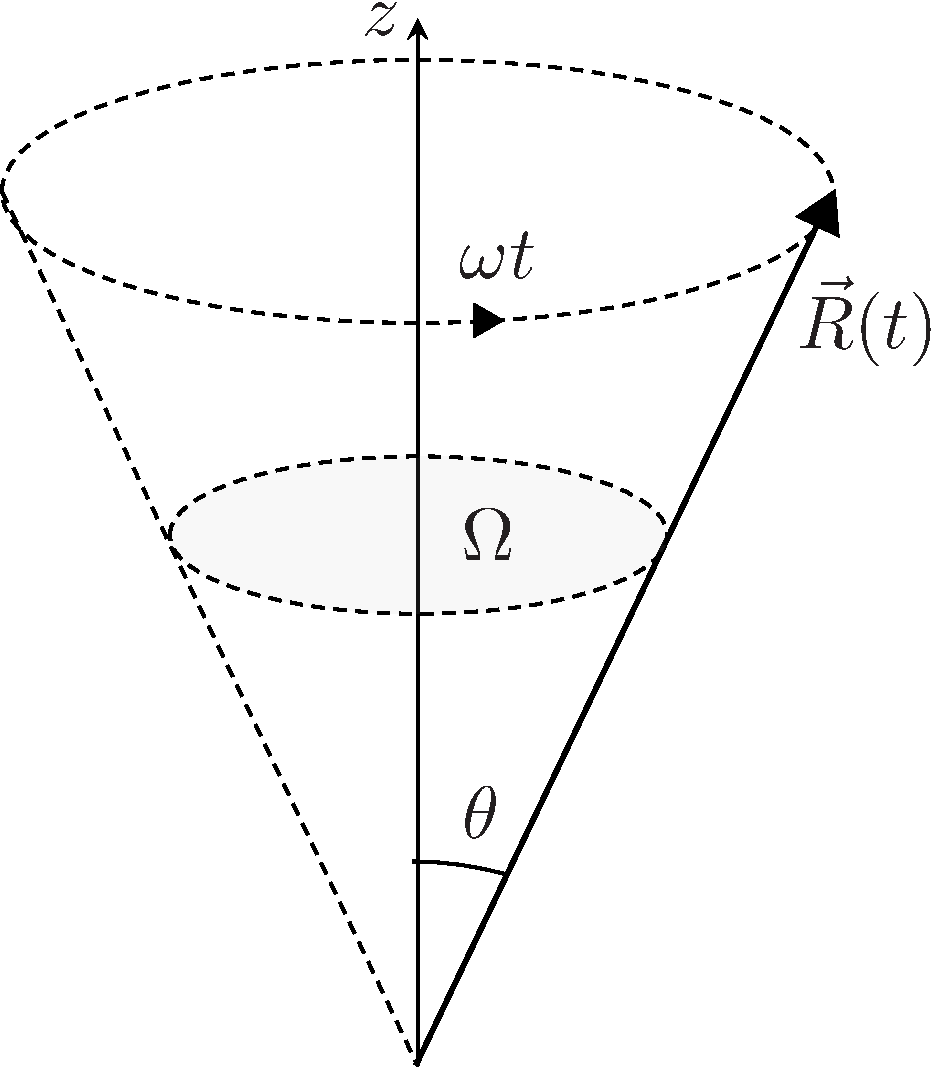
\includegraphics[width=0.9\textwidth]{Figures/RotatingVector-crop.pdf}
\end{minipage}

$\hat{R}(t)$ is a unit vector $\rightarrow$ parameter space of the
environment is \emph{unit sphere}.
An example is the field precessing with
frequency $\omega$ about the $\hat{z}$ direction:
\be
\vec{R}(t)=\hat{x} \sin \theta \cos (\phi+\omega t)+ \hat{y} \sin \theta \sin (\phi+\omega t)+\hat{z} \cos \theta
\label{eq:g81}
\ee
(counter clockwise precession)

%%% 02 OKAY

The state of the system, $|\psi(t)\rangle$, is described by the
Schrödinger equation:
\be
i\hbar \frac{d|\psi(t)\rangle}{d t}=\hat{H}(R)|\psi(t)\rangle
\label{eq:g82}
\ee
We consider as the physical Hilbert space of states $H$,
the space that contains the solution of Eq.~\eqref{eq:g82}
for all possible values of $\vec{R}$ in the parameter
space. Then, for any value of $\vec{R}$, one may
choose an orthonormal basis of eigenvectors
$\ket{n;R}$ of the parameter-dependent Hamiltonian:
\be
\begin{gathered}
\hat{H}(R)|n ; R\rangle=E_{n}(R)|n ; R\rangle\\
\langle m ; R \mid n ; R\rangle=\delta_{m n}
\end{gathered}
\label{eq:g83}
\ee
so
\be
\hat{H}(R)=\sum_{n} E_{n}(R) \hat{P}_{n}(R)
\ee
where
\be
\hat{P}_{n}(R)=|n ; R\rangle\langle n ; R|
\ee
Here and in the rest of the discussion, we assume that
the Hamiltonian has a discrete spectrum.

%%% 03 OKAY

Given an environmental process along with a time
parametrization, $R \rightarrow R(t)$, one obtains a time-dependent
Hamiltonian, $\hat{H}(R) \rightarrow \hat{H}(t)$, with $\hat{H}(t)$ having a
spectral representation
\be
\hat{H}(t)= \sum_n E_{n}(R(t)) \hat{P}_{n}(R(t))
\ee
with
\be
\hat{P}_{n}(R(t))=|n ; R(t)\rangle\langle n ; R(t)|
\ee
where $E_{n}(R(t)),\,|n ; R(t)\rangle$ are the instantaneous eigenvalues
and eigenvectors.

\emph{Note that:} Single-valuedness of $\hat{H}$ and $\hat{A}$ does not
inply that $|h, R\rangle$ are single-valued functions
of $\vec{R}$. For example: periodic environment, \textit{i.e}.
$\vec{R}(0)=\vec{R}(T)$, a closed path $C$, one can have
\be
|n ; R(T)\rangle=e^{i \alpha}|n, R(0)\rangle
\ee
$\rightarrow$ example is rotation of spin-1/2.

In general, you can make a \emph{gauge transformation}:
\be
|n ; R\rangle \rightarrow|n, R\rangle^{\prime}=e^{i \phi_{n}(R)}|n, R\rangle
\label{eq:g89}
\ee
Assumption: $\phi_{n}(R)$ are single-valued functions of $\vec{R}(t)$.

%%% 04 OKAY

The solution of the Schrödinger equation in Eq.~\eqref{eq:g82}
\be
|\psi(t)\rangle=\hat{U}(t)|\psi(0)\rangle
\ee
with
\be
\hat{U}(t) = T e^{-1 / \hbar \int_{0}^{t} d t^{\prime} \hat{H}(t)}, \quad \hat{H}(t)=\hat{H}(\vec{R}(t))
\ee
Now, if
\be
\left[\hat{H}(t), \hat{H}\left(t^{\prime}\right)\right]=0
\label{eq:g92}
\ee
the $\hat{U}(t)$ can be written as
\be
\hat{U}(t)=e^{-i / \hbar \int_{0}^{t} d t^{\prime} \hat{H}(t^\prime)}
\ee
Suppose that $|\psi(0)\rangle=|n, R(0)\rangle$, \textit{i.e.} it is an
eigenstate of $\hat{H}(R(0))$. Then:
\be
\ket{\psi(t)}=e^{-i / \hbar \int_{0}^{t} d t^{\prime} E_n(R(t))}\ket{\psi(0)}
\ee
Eq.~\eqref{eq:g92}, in general, is a too drastic assumption
(or approximation): the interaction with the environment,
described by a time-dependent $\hat{H}(R(t))$ makes
the system to jump from the $n$-th eigenstate
$|n, R(0)\rangle\langle n, R(0)|$ at $t=0$ into any other eigenstate
%%% 04 prime (faltando nas notas, tirei do vídeo)
$|m, R(t)\rangle\langle m, R(t)|, m \neq n$, at a later time $t$
(remember, \textit{e.g.}, our studies about magnetic resonance in two-level systems).

BUT, it might happen that the system
remains an eigenstate of $\hat{H}(R(t))$ at all
times with the same quantum number $n$,
\textit{i.e.} it does not jump to another with $m$:
\be
\begin{aligned}
t=0, \quad&|\psi(0)\rangle=|n, R(0)\rangle\\
t=t, \quad&|\psi(t)\rangle=|n, R(t)\rangle
\end{aligned}
\ee
so
\be
|\psi(t)\rangle\langle\psi(t)|=| n ; R(t)\rangle\langle n ; R(t)|=P_{n}(R(t))
\label{eq:g96}
\ee
or
\be
\hat{\rho}(t)=P_{n}(R(t))
\ee
This is known as the \emph{adiabatic time development},
which is a generalization of the condition that
a state is \emph{stationary}, \textit{i.e.}
\be
\hat{\rho}(t)=|\psi(t)\rangle\langle\psi(t)|=| \psi(0)\rangle\langle\psi(0)|
\ee

\emph{Next:} we will see that 
Eq.~\eqref{eq:g96} is an
approximation, \textit{i.e.} it cannot be an exact
statement!
\end{document}
















































